%-------------------------------- Configurações --------------------------------

\documentclass[a4paper,         % Tamanho do papel: A4
	           abntfigtabnum,
	           noindentfirst,
	           normaltoc,
	           pnumplain,
	           notimes
	           % capchap,
]{abnt}

% Links border color
\newcommand{\bc}{NavyBlue}

\usepackage[utf8]{inputenc} % para pode escrever caracteres acentuados normalmente
\usepackage[brazil]{babel}
\usepackage{graphicx}
\usepackage[usenames,dvipsnames]{xcolor} % http://en.wikibooks.org/wiki/LaTeX/Colors
\usepackage[pdfborder={0 0 0},pdfborderstyle={/S/U/W 0.5},citebordercolor=\bc,filebordercolor=\bc,urlbordercolor=\bc,linkbordercolor=\bc]{hyperref} % http://www.tug.org/applications/hyperref/manual.html e http://migre.me/7FH3e
\usepackage[alf]{abntcite}
\usepackage{booktabs} % para utilização das linhas separadoras na tabela
\usepackage{textcomp}
\usepackage{minted} % foi adicionado o seguinte hack no minted: http://migre.me/7M8wI

%--------------------------- Minted Highligthing -------------------------------

\renewcommand\listingscaption{Código}

% http://github.com/hugomaiavieira/pygments-style-github
\usemintedstyle{github}

% O minted é tipo uma extensão do fancyvrb. Então, algumas modificações nele
% são feitas de acordo com o fancyvrb.
% Documentação do fancyvrb: http://linorg.usp.br/CTAN/macros/latex/contrib/fancyvrb/fancyvrb.pdf

% Ajustar o estilo do número, de acordo com o fancyvrb.
\renewcommand{\theFancyVerbLine}{\textcolor{Gray}{\scriptsize\arabic{FancyVerbLine}}}

% Ajusta estilo do caption. http://linorg.usp.br/CTAN/macros/latex/contrib/caption/caption-eng.pdf
\usepackage{caption}
\DeclareCaptionStyle{code_style}{justification=centering, skip=20pt}
\captionsetup[listing]{style=code_style}

% Criando um novo comando para facilitar a adição de códigos
% http://tex.stackexchange.com/questions/42393/new-environment-with-minted
\makeatletter
\newenvironment{mycode}[3]
 {\VerbatimEnvironment
  \minted@resetoptions
  \setkeys{minted@opt}{linenos,fontfamily=courier, fontsize=\scriptsize, xleftmargin=21pt, frame=lines, framesep=5pt, framerule=1pt, numbersep=4pt}
  \renewcommand{\minted@proglang}[1]{#1}
    \captionof{listing}{#2\label{#3}} % http://migre.me/85CIT
      \begin{VerbatimOut}{\jobname.pyg}}
 {\end{VerbatimOut}
  \minted@pygmentize{\minted@proglang{}}
  \DeleteFile{\jobname.pyg}}
\makeatother

%--------------------------------- Informações ---------------------------------

% http://www.tug.org/applications/hyperref/manual.html
\hypersetup{
  pdftitle=Técnicas emergentes de desenvolvimento de software,
  pdfauthor=Hugo Henriques Maia Vieira
  % pdfsubject={},
}

\begin{document}

\titulo{Técnicas emergentes de desenvolvimento de software}
\autor{Hugo Henriques Maia Vieira}
\instituicao{Universidade Estadual do Norte Fluminense Darcy Ribeiro\par Laboratório de Ciências Matemáticas}
\orientador{Rodrigo Soares Manhães, M.Sc.}
\comentario{Monografia apresentada ao Curso de Graduação em Ciência da
Computação da Universidade Estadual do Norte Fluminense Darcy Ribeiro como
requisito para obtenção do título de Bacharel em Ciência da Computação, sob
orientação do Prof. Rodrigo Soares Manhães, M.Sc.}
\local{Campos dos Goytacazes/RJ}
\data{2012}


\capa
\folhaderosto


% Adiciona linha acima dos nomes para a assinatura na folha de aprovação
\setlength{\ABNTsignthickness}{0.4pt}
% Adiciona um espaçamento maior entre os nomes na folha de aprovação
\setlength{\ABNTsignskip}{3cm}

\begin{folhadeaprovacao}
  Monografia apresentada ao Curso de Graduação em Ciência da
Computação da Universidade Estadual do Norte Fluminense Darcy Ribeiro como
requisito para obtenção do título de Bacharel em Ciência da Computação, sob
orientação do Prof. Rodrigo Soares Manhães, M.Sc.

  \assinatura{Prof. M.Sc. Rodrigo Soares Manhães \\ Orientador}

  \assinatura{Profª. Drª. Annabell del Real Tamariz \\ Universidade Estadual do Norte Fluminense Darcy Ribeiro}

  \assinatura{Prof. Dr. Rogério Atem de Carvalho \\ Instituto Federal Fluminense}
\end{folhadeaprovacao}


\begin{titlepage}
 \vspace*{5cm}
 \begin{flushright}
  ``As pessoas boas devem amar seus inimigos''\\\textit{Seu Madruga}
  \vspace{1cm}
 \end{flushright}
\end{titlepage}


\begin{center}
\textbf{AGRADECIMENTOS} \\ [2.5cm]
\end{center}

A meu pai, minha mãe e especialmente a você.



\listoffigures

\begin{resumo}
Aqui entra o resumo do meu trabalho que será a última coisa a ser feita.
\end{resumo}

\begin{abstract}
Write here the English version of your ``Resumo".
\end{abstract}

\sumario

\chapter{Introdução}

O desenvolvimento de software passou, e de certa forma ainda passa, por uma fase conhecida como \emph{crise do software}, termo utilizado pela primeira vez por \citeonline{HumbleProgrammer}. A Engenharia de Software surgiu \cite{NaurRandell} numa tentativa de contornar esta crise. No entanto, a ela foi baseada em algumas considerações equivocadas, que serão abordadas posteriormente, fazendo com que falhasse na sua tentativa de contornar tal crise.

Com o passar dos anos, o mercado demanda e espera software inovadores e de alta qualidade, que sejam adequados a suas necessidades – e o mais rápido possível \cite{TheBusinessOfInnovation}. Como isso não foi praticável através do Engenharia de Software tradicional, buscou-se uma abordagem alternativa.

O desenvolvimento ágil de software, que neste ano de 2012 completa 11 anos, foi elaborado \cite{AgileManifesto} para resolver esta crise que a Engenharia de Software tradicional não conseguiu, focando nas pessoas ao invés do processo e abraçando as mudanças ao invés de evitá-las. De acordo com \citeonline{PMNetworkFailureDrop}, o \textit{Chaos Manifesto 2011}\footnote{O \textit{Chaos Manifesto} é uma pesquisa bienal realizada pelo \textit{The Standish Group} e teve início em 1994. As pesquisas publicadas em um ano representam os dados do ano anterior.} mostra que os resultados de 2010 representam, desde sua primeira edição, a maior taxa de sucesso nos projetos de desenvolvimento de software, que aumentou de 32\% em 2008 para 37\% em 2010. Segundo \citeonline{ResumoChaosReport}, o \textit{The Standish Group} conclui que uma das principais razões para o aumento da taxa de sucesso foi a utilização das metodologias ágeis, que cresce a uma taxa de 22\% CAGR\footnote{\href{http://en.wikipedia.org/wiki/Compound_annual_growth_rate} {Compound annual growth rate}} e hoje são adotados em 9\% de todos os projetos de TI em andamento e em 29\% dos novos projetos.

Como o desenvolvimento ágil é relativamente novo, diversos métodos e técnicas vem sendo desenvolvidos tendo como base os princípios e valores ágeis \cite{BDDRodrigo}. Sendo técnicas emergentes, ainda são pouco discutidas no meio acadêmico, este trabalho pretende contribuir com esta discussão e, de certa forma, com a introdução de técnicas vindas do mercado na academia.


\section{Objetivos}

O objetivo principal do presente trabalho é contribuir com a introdução de técnicas e discussões surgidas no mercado para a academia, além de compilar informações, hoje dispersas, sobre as vantagens e desvantagens da utilização de tais técnicas.

Existem também algumas questões em aberto no desenvolvimento ágil de software, que serão alvo de discussão neste trabalho.

\section{Metodologia}

Será feita uma explanação sobre cada técnica e uma discussão mostrando onde são melhor aplicadas, comparando as diferentes abordagens para cada técnica, bem como as vantagens e desvantagens em seu uso.

Como base para a discussão, será utilizado o kanban-roots\footnote{\url{http://github.com/hugomaiavieira/kanban-roots}}, que está sendo desenvolvido em conjunto com o presente trabalho.

O kanban-roots é um kanban\footnote{O termo tem origem no sistema Toyota de produção, onde kanban é a maneira como é coordenado o fluxo de peças na cadeia de suprimentos  \cite{AMaquinaQueMudouOMundo}. No contexto do presente trabalho, kanban é um quadro para visualização do fluxo de trabalho (tarefas) em um projeto.} online para auxiliar a organização e acompanhamento das tarefas em um projeto. O kanban-roots já está em produção e vem sendo testado e utilizado com sucesso por algumas pessoas e empresas, não só do Brasil, mas também da França, Lituânia, Polônia, Africa do Sul, Rússia, Inglaterra, China, Finlândia, Peru, Estados Unidos, entre outros.

Na figura \ref{img:tela_kaban_roots} pode ser visto um \textit{print} da tela do kanban de um projeto no kanban-roots.

\begin{figure}[h]
  \center
  \caption{Tela do kanban de um projeto no kanban-roots}
  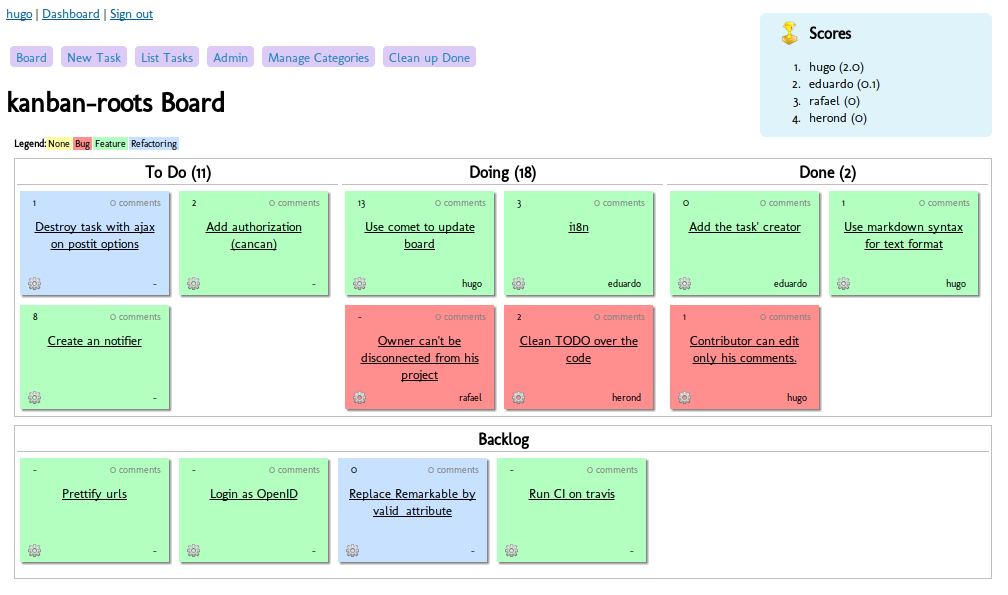
\includegraphics[scale=0.45]{images/kanban-roots}
  \label{img:tela_kaban_roots}
\end{figure}

Todos os trechos de código apresentados neste trabalho são trechos retirados do kanban-roots. A primeira linha de cada trecho sempre é um comentário informando o nome do arquivo original.

\section{Ferramentas}

Para o desenvolvimento do kanban-roots foram utilizadas diversas ferramentas, sendo importante citar em que contexto e momento cada uma delas é utilizada.

Como base para o desenvolvimento, foi utilizado o \textit{framework web} \textit{Ruby On Rails}\footnote{\url{http://rubyonrails.org}}. Para os testes de unidade apresentados na seção \ref{sec:tdd} foi utilizado o \textit{Test::Unit}\footnote{\url{http://test-unit.rubyforge.org/}}. Já na seção \ref{sec:bdd} é utilizado o \textit{Rspec}\footnote{\url{http://rspec.info/}} para testes unitários, testes de aceitação e dublês de teste. Ainda na seção \ref{sec:bdd} também foi utilizado o \textit{Cucumber}\footnote{\url{http://cukes.info/}} para testes de aceitação. Além dessas ferramentas, também foi utilizado o \textit{FactoryGirl}\footnote{\url{https://github.com/thoughtbot/factory_girl}} para \textit{fixtures replacement} em todos os momentos em que se fez necessário.
\chapter{Fundamentação teórica}

\section{Agilismo}
\label{sec:agilismo}

Em 2001 um grupo de dezessete especialistas, reconhecidos pela comunidade como grandes nomes do desenvolvimento software, se reuniram para discutir sobre um crescente conjunto de métodos que vinham surgindo e decidiram usar o termo Agilismo para descrever essa nova geração de métodos ágeis \cite{AgileStory}. Na mesma reunião, eles também escreveram o Manifesto Ágil \cite{AgileManifesto}, delineando um conjunto de valores e princípios que, em resumo, trilham um caminho para a eliminação de documentação e processos desnecessários, buscando a simplicidade, com foco na geração de valor e proximidade com o cliente, além de possibilitar respostas rápidas e eficazes às mudanças.

Pode-se dizer então, que o Desenvolvendo Ágil, ou Agilismo, é um rótulo genérico para os métodos de desenvolvimento de software baseados no Manifesto Ágil \cite{BDDRodrigo}.

% section agilismo (end)

\section{Tipos de teste}
\label{sec:tipos_de_teste}

\subsection{Testes de unidade}
\label{sub:testes_de_unidade}

Testes de unidade são testes nos quais unidades individuais do sistema são testadas para determinar se estão aptas para uso. Uma unidade é a menor parte testável de uma aplicação. Em programação procedural uma unidade pode ser uma função ou \textit{procedure}. Já em programação orientada a objetos, uma unidade pode ser um método.

% subsection testes_de_unidade (end)

\subsection{Testes de integração}
\label{sub:testes_de_integracao}

Teste de integração testam as integrações do código com o mundo exterior. Podem ser um teste que se comunique através da rede, tenha contato com o sistema de arquivos ou deixe os limites de seu próprio processo \cite{ArtOfAgileDevelopment}.

% subsection testes_de_integracao (end)

\subsection{Testes de aceitação}
\label{sub:testes_de_aceitacao}

Testes de aceitação são especificações para o comportamento e funcionalidade de um sistema. Os testes de aceitação nos mostram se o sistema se comporta corretamente pela perspectiva de um usuário, sem nos dizer nada sobre como o sistema implementa esse comportamento \cite{TestDrivenKoskela}.

% subsection testes_de_aceitacao (end)

% section tipos_de_teste (end)
\chapter{Técnicas}

\section{Test-Driven Development (TDD)}
\label{sub:tdd}
``Apenas escrever código para corrigir um teste falhando". Segundo \citeonline{TestDrivenKoskela}, isto é \textit{Test-Driven Development} (Desenvolvimento guiado por testes) \cite{TDDbyExample} em apenas uma sentença.

O TDD é uma técnica onde o desenvolvimento do software é guiado por \textbf{testes automatizados}, que são escritos antes de qualquer linha de código relativo a funcionalidades. Primeiro escreve-se um teste, depois escreve-se o código para passar neste teste. Em seguida, o código é refatorado para encontrar um design melhor, contando sempre com os testes existentes para que não sejam introduzidas falhas em outras partes do sistema.

Esta abordagem encoraja bom design \cite{GrowingOOByTests}, produz código testável e mantém longe a sobre-engenharia por conta de falsas suposições, pois, nos testes, é especificado o que é desejado e escreve-se o código para fazer apenas aquilo que realmente é necessário. \cite{TestDrivenKoskela, TDDbyExample, EmpiricalTDD}

Mas TDD é uma técnica emergente? Não e sim.

O TDD vem sendo utilizado esporadicamente há anos, contudo, não existia um nome para identificar essa forma de desenvolver software. Além disso, em termos de adoção, TDD continua sendo novo \cite{TestDrivenKoskela, TDDbyExample, EmpiricalTDD}. Hoje, esta técnica tem um nome e começa a ganhar força, sendo utilizada em times de grandes empresas como Google, Yahoo, Microsoft e IBM \cite{EmpiricalTDD}.

\subsection{Ciclo TDD}
\label{ssub:ciclo_tdd}

Com base no trabalho de \citeonline{TDDbyExample}, o ciclo de desenvolvimento TDD é composto pelas seguintes etapas:

\begin{enumerate}
\item \textbf{Adicionar um teste}

Cada ciclo se inicia com a criação de um teste de unidade. Este teste inevitavelmente irá falhar, pois é escrito antes do código ser implementado de fato. Para escrever um teste, o desenvolvedor precisa entender claramente as especificações e requisitos da unidade. Isso faz com que o desenvolvedor tenha como foco os requisitos antes do código, o direcionando a escrever código apenas para o que é realmente necessário.

\item \textbf{Executar todos os testes e ver se algum falha}

Todos os testes devem ser executados e o novo teste deve falhar pela razão esperada: a funcionalidade não foi desenvolvida. Isto aumenta a confiança que se está testando a coisa certa.

\item \textbf{Escrever código}

O próximo passo é escrever código \textbf{somente para que o teste passe}. O código poderá não ser perfeito, pois posteriormente ele será melhorado. O importante é que o código faça o mínimo para passar no teste. Segundo \citeonline{BDDRodrigo}:

\begin{citacao}
Enquanto código útil é um patrimônio que gera valor, qualquer código criado inutilmente é tempo desperdiçado e, no fim das contas, um fardo, que sem gerar valor algum, aumentará a complexidade geral do software.
\end{citacao}

\item \textbf{Executar os testes e ter sucesso}

Ao Executar os testes e todos eles passarem, o código possuirá todos os requisitos testados e o programador pode ficar confiante para melhorá-lo.

\item \textbf{Refatorar}

Esta é uma etapa muito importante, onde o código escrito anteriormente é melhorado.

Segundo \citeonline{FowlerRefatoracao}, refatorar é reestruturar o software aplicando uma série de alterações em sua estrutura interna para torná-lo mais fácil de ser entendido e menos custoso de ser modificado, sem alterar seu comportamento observável.

Refatorar melhora o projeto do software, o torna mais fácil de entender e modificar, ajuda a encontrar falhas e ajuda o desenvolvedor a programar mais rapidamente.

Como na refatoração o comportamento do código não deve ser alterado, após refatorar e executar novamente os testes, todos eles devem passar.

\end{enumerate}

A figura \ref{img:ciclo-tdd} resume o ciclo TDD de forma bem clara.

\begin{figure}[h]
  \center
  \caption{O ciclo TDD}
  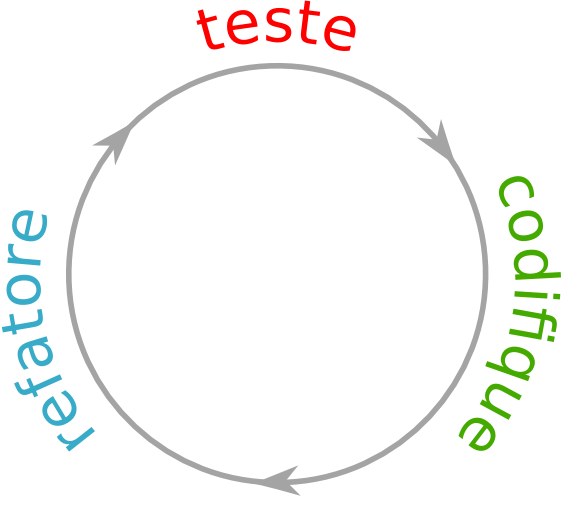
\includegraphics[scale=0.45]{images/ciclo-tdd}
  \label{img:ciclo-tdd}
\end{figure}

\subsection{TDD na prática}
\label{ssub:tdd_na_pratica}

Vejamos agora como isso se dá na prática através de um exemplo retirado do código do kanban-roots.

A seguinte funcionalidade precisa ser implementada:

\begin{quote}
\textit{Precisa-se saber todas as tarefas em uma determinada posição do kanban de um projeto.}
\end{quote}

A primeira coisa a ser feita é o teste para o caso mais simples: quando o projeto não tem tarefa alguma naquela determinada posição.

Desta forma, o teste para o caso mais simples pode ser como mostrado no código \ref{code:tdd_test1}.

\begin{mycode}{ruby}%
{Teste para o método Project\#tasks\_by\_position (versão 1)}{code:tdd_test1}
# test/unit/project_test.rb
class ProjectTest < ActiveSupport::TestCase
  def test_tasks_by_position
    project = Factory.create :project
    assert_equal(project.tasks_by_position(4), [])
  end
end
\end{mycode}

Ao rodar este teste, ele irá falhar, informando que o método \textit{tasks\_by\_position} sequer existe. Como esta era a falha esperada, escrevemos então o código mais simples para passar neste teste, apresentado no código \ref{code:tdd_code1}.

\begin{mycode}{ruby}%
{Código do método Project\#tasks\_by\_position (versão 1)}{code:tdd_code1}
# app/models/project.rb
def tasks_by_position position
  []
end
\end{mycode}

Os testes irão passar. Mas a funcionalidade ainda não está completa e, consequentemente, o teste também não. Como pode ser visto no código \ref{code:tdd_test2}, é adicionado ao teste uma verificação de que para a posição 1 devem existir duas tarefas e que estas tarefas devem ser exatamente as criadas anteriormente.

\begin{mycode}{ruby}%
{Teste do método Project\#tasks\_by\_position (versão 2)}{code:tdd_test2}
# test/unit/project_test.rb
class ProjectTest < ActiveSupport::TestCase
  def test_tasks_by_position
    project = Factory.create :project
    tasks = [Factory.create(:task, :project => project, :position => 1),
             Factory.create(:task, :project => project, :position => 1)]

    assert_equal(project.tasks_by_position(4), [])

    assert_equal(project.tasks_by_position(1).count, 2)
    tasks.each { |task| assert(project.tasks_by_position(1).include?(task)) }
  end
end
\end{mycode}

Como o teste foi alterado, este é executado e irá falhar, informando que na \hyperref[code:tdd_test1]{linha 10} eram esperadas duas tarefas, mas foram obtidas zero. O código então deve ser modificado para passar no novo teste e é apresentado no código \ref{code:tdd_code2}.

\begin{mycode}{ruby}%
{Código do método Project\#tasks\_by\_position (versão 2)}{code:tdd_code2}
# app/models/project.rb
def tasks_by_position position
  task_list = []
  tasks.each do |task|
    task_list << task if task.position.to_s == position.to_s
  end
  task_list
end
\end{mycode}

Desta vez, após a modificação no código e a execução dos testes, todos os testes os irão passar. Contudo, a cobertura de testes para este método ainda está fraca, o que pode ser resolvido com a adição de mais algumas tarefas em posições diferentes, como mostrado no código \ref{code:tdd_test3}.

\begin{mycode}{ruby}%
{Teste do método Project\#tasks\_by\_position (versão 3)}{code:tdd_test3}
# test/unit/project_test.rb
class ProjectTest < ActiveSupport::TestCase
  def test_tasks_by_position
    project = Factory.create :project
    tasks = [Factory.create(:task, :project => project, :position => 1),
             Factory.create(:task, :project => project, :position => 1),
             Factory.create(:task, :project => project, :position => 2),
             Factory.create(:task, :project => project, :position => 3),
             Factory.create(:task, :project => project, :position => 3)]

    assert_equal(project.tasks_by_position(4), [])

    assert_equal(project.tasks_by_position(1).count, 2)
    tasks[0..1].each { |task| assert(project.tasks_by_position(1).include?(task)) }

    assert_equal(project.tasks_by_position(2), [tasks[2]])

    assert_equal(project.tasks_by_position("3").count, 2)
    tasks[3..4].each { |task| assert(project.tasks_by_position("3").include?(task)) }
  end
end
\end{mycode}

Executando os testes novamente, todos eles passam. Isto indica que já é hora de ir para o item 5 do ciclo TDD e refatorar. Ao comparar o Código \ref{code:tdd_code2} com o Código \ref{code:tdd_code3}, pode-se perceber como o Código \ref{code:tdd_code3} está mais simples e claro e que ao rodar os testes, estes passam mostrando que o comportamento do método não mudou.

\begin{mycode}{ruby}%
{Código do método Project\#tasks\_by\_position (versão 3)}{code:tdd_code3}
# app/models/project.rb
def tasks_by_position position
  tasks.select { |item| item.position.to_s == position.to_s }
end
\end{mycode}

\citeonline{TDDAntiPatterns} descreve vários anti-padrões do TDD e sua leitura é fortemente recomendada.

\subsection{Design emergente} % (fold)
\label{sub:design_emergente}

No contexto em que TDD costuma ser aplicado – em processos ágeis, com um ciclo de vida iterativo-incremental – não é realizado um amplo \textit{design} prévio. Sendo assim, o \textit{design} evolui incrementalmente. Sabendo disso, uma característica extremamente importante do TDD é a facilitação ao \textit{design} emergente, que muitos consideram ser sua a principal característica.

\textbf{TODO: dar um exemplo do kanban (ver histórico de commits no github) e PROCURAR REFERÊNCIAS SOBRE ISSO}

% subsection design_emergente (end)


\section{Behaviour-Driven Development (BDD)}
\label{sec:bdd}

Criado em 2006 \cite{IntroducingBDD}, \textit{Behaviour-Driven Development} (Desenvolvimento guiado por comportamento) é uma técnica de desenvolvimento de software cuja amplitude se estende às atividades de design, documentação, validação e verificação, tratando-as de modo unificado \cite{BDDRodrigo}.

\subsection{A herança de TDD}
\label{sub:a_heranca_de_tdd}

O BDD é uma evolução do TDD. A grande diferença entre os dois é que TDD não abrange a validação do software, ou seja, se o software atende os requisitos. Isso muda tudo, pois em BDD, a ênfase está no comportamento, e não na estrutura. Ao invés de focar em classes e métodos ao escrever os testes, o foco é no comportamento que gera valor para o sistema. Além disso, o pensamento não é voltado à verificação, mas sim no comportamento, em validar que o software faz sem deixar também de verificar se está funcionando como deveria.

Em BDD não são escritos testes, mas sim especificações, chamadas de \textit{specs} (de \textit{specifications}). Pode-se ter a clara diferença comparando o Código \ref{code:tdd_test3} com o Código \ref{code:bdd_spec}, onde palavras chave como \textit{class}, \textit{test} e \textit{assert} dão lugar a \textit{describe}, \textit{it} e \textit{should}, e fica nítido o foco no comportamento, inclusive nas asserções.

\begin{mycode}{rspec}%
{Spec}{code:bdd_spec}
# spec/models/project.rb
describe Project do
  it "returns all related tasks matching a given position" do
    project = Factory.create :project
    tasks = [Factory.create(:task, :project => project, :position => 1),
             Factory.create(:task, :project => project, :position => 1),
             Factory.create(:task, :project => project, :position => 2),
             Factory.create(:task, :project => project, :position => 3),
             Factory.create(:task, :project => project, :position => 3)]

    project.tasks_by_position(4).should be_empty

    project.should have(2).tasks_by_position(1)
    project.tasks_by_position(1).should include(*tasks[0..1])

    project.tasks_by_position(2).should == [tasks[2]]

    project.should have(2).tasks_by_position(3)
    project.tasks_by_position(3).should include(*tasks[3..4])
  end
end
\end{mycode}

Em TDD, o nome dos testes é baseado na estrutura do código, e isso pode ter um efeito colateral: criar duplicações. Ao escrever testes como o do Código \ref{code:tdd_test3} \textit{test\_tesks\_by\_position} e o método \textit{tasks\_by\_position} é renomeado, o nome do teste também terá que ser renomeado, o que provavelmente é esquecido. Isso torna os testes confusos e desinformativos \cite{ContinuousTesting}. Como por definição, refatorar é melhorar a estrutura e o design do código sem alterar seu comportamento, nomeando os testes com base no comportamento desejado ao invés da estrutura do código, não apenas torna os testes mais informativos como também torna a refatoração menos custosa \cite{ContinuousTesting}.

% subsection a_heranca_de_tdd (end)

\subsection{O ciclo BDD}
\label{sub:o_ciclo_bdd}

O Ciclo BDD, apresentado na Figura \ref{img:ciclo-bdd}, tem dois níveis: unidade e aceitação. O nível aceitação é o nível mais alto, onde são escritos os testes de aceitação. Já o nível unidade é o mesmíssimo ciclo TDD visto anteriormente.

\begin{enumerate}
\item \textbf{Adicionar um teste de aceitação}

Cada ciclo se inicia com a criação de um teste de aceitação, um cenário, que descreve um determinado comportamento de uma funcionalidade do sistema.

\item \textbf{Executar todos os testes e ver se algum falha}

Todos os testes devem ser executados e o novo teste deve falhar pela razão esperada: a funcionalidade não foi desenvolvida. Isto aumenta a confiança que se está testando a coisa certa.

\item \textbf{Descer de nível}

Neste momento, deve-se descer de nível, saindo do nível de aceitação e indo para  nível de unidade.

\item \textbf{Entra no ciclo TDD}

No nível de unidade, entra-se o ciclo TDD até que todos os testes de unidade estejam passando.

\item \textbf{Retornar para o nível de aceitação}

Com todos os testes de unidade passando, retorna-se para o nível de aceitação e faz-se todos os testes passarem.

\item \textbf{Refatorar}

Refatora-se o código.

\end{enumerate}

\begin{figure}[h]
  \center
  \caption{O ciclo BDD}
  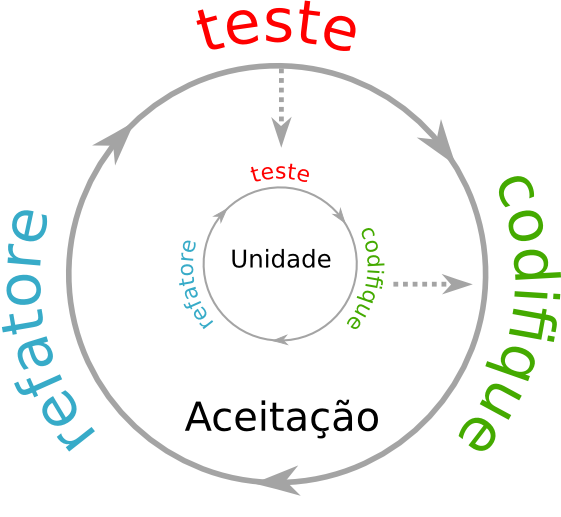
\includegraphics[scale=0.45]{images/ciclo-bdd}
  \label{img:ciclo-bdd}
\end{figure}

% subsection o_ciclo_bdd (end)

\subsection{Modelos de escrita dos testes de aceitação}
\label{sub:modelos_de_escrita_dos_testes_de_aceitacao}

Existem duas maneiras de se escrever os testes de aceitação: em texto plano e em código puro. Para exemplificar cada um das abordagens, será especificada a seguinte funcionalidade:

\begin{quote}
\textit{Os comentários mostrados na página de tarefas devem ser renderizados utilizando a linguagem de marcação Markdown.}
\end{quote}

\subsubsection{Escrita em texto plano} % (fold)
\label{subsub:escrita_em_texto_plano}

Uma das maneiras de escrever testes de aceitação é como texto plano, ou seja, inglês, português e etc. Nas ferramentas que implementam esta abordagem, os testes são escritos baseados em \textit{steps} (passos), onde cada step é mapeado para um código real.

No código \ref{code:bdd_cucumber_spec}, é utilizado o \textit{cucumber} para fazer a especificação. Como pode-se ver, o teste é escrito em linguagem que qualquer pessoa, mesmo sem nenhum conhecimento em programação, pode ler e validar.

\begin{mycode}{cucumber}%
{Especificação em texto plano}{code:bdd_cucumber_spec}
# features/comments.feature
Feature: Render comments with Markdown syntax
  As a user
  I want to use Markdown in my comments
  In order to make my comments more expressives

  Scenario: on tasks page
    Given I am a contributor of "sgtran" project
    And I am authenticated
    And I have a task of "sgtran" project
    When I am on the task page
    And I fill in "comment_content" with "# Some content [link](http://exemplo.com)"
    And I press "Comment"
    Then I should see "Some content" in a "h1" tag
    And I should see "link" in an "a" tag
\end{mycode}

Para cada \textit{step} existe uma implementação, ou seja, sua definição, chamada de \textit{step definition}. Pode-se pensar nos \textit{steps} como chamadas à métodos, e assim, os \textit{step definitions} serão as definição desse métodos. Os \textit{step definitions} para os \textit{steps} do código \ref{code:bdd_cucumber_spec} são apresentado no código \ref{code:step_definition}.

Como durante o desenvolvimento são escritos muitos \textit{step definitions}, com o intuito de organizá-los, eles são separados por contexto em arquivos diferentes.

\begin{mycode}{ruby}%
{Step definitions}{code:step_definition}
# features/step_definitions/contributor_steps.rb
Given /^I am a contributor of "([^"]*)" project$/ do |name|
  @project = Factory.create :project, :name => name
  @contributor = Factory.create :contributor, :contributions => [@project]
  @project.update_attribute(:contributors, [@contributor])
end

# features/step_definitions/contributor_steps.rb
Given /^I am(?:| an) authenticated(?:| contributor)$/ do
  @contributor ||= Factory.create :contributor

  Given %{I am on the sign in page}
  And %{I fill in "contributor_login" with "#{@contributor.email}"}
  And %{I fill in "contributor_password" with "#{@contributor.password}"}
  And %{I press "Sign in"}
end

# features/step_definitions/task_steps.rb
Given /^I have a task of "([^"]*)" project$/ do |project_name|
  @project = Factory.create :project, :name => 'project_name'
  @task = Factory.create :task, :project => @project, :author => @contributor
end

# features/step_definitions/web_steps.rb
Given /^(?:|I )am on (.+)$/ do |page_name|
  visit path_to(page_name)
end

# features/step_definitions/web_steps.rb
When /^(?:|I )fill in "([^"]*)" with "([^"]*)"$/ do |field, value|
  fill_in(field, :with => value)
end

# features/step_definitions/web_steps.rb
When /^(?:|I )press "([^"]*)"$/ do |button|
  click_button(button)
end

# features/step_definitions/my_web_steps.rb
When /^I should see "([^"]*)" in a(?:|n) "([^"]*)" tag$/ do |text, tag|
  if page.respond_to? :should
    page.should have_xpath("//#{tag}", :text => text)
  else
    assert page.has_xpath?("//#{tag}", :text => text)
  end
end
\end{mycode}

% subsubsection escrita_em_texto_plano (end)


\subsubsection{Escrita em código puro} % (fold)
\label{subsub:Escrita em codigo puro}

A outra maneira de escrever os testes de aceitação é com código puro. Nesta forma, todo o código dos testes está concentrado em apenas um lugar, utilizando somente código para escrever os testes.

No código \ref{code:bdd_spec1} pode-se ver a especificação em código puro para a funcionalidade.

\begin{mycode}{rspec}%
{Especificação}{code:bdd_spec1}
# spec/acceptance/comments_spec.rb
feature "Render comments with Markdown syntax" do
  background do
    @owner = Factory.create :contributor
    @project = Factory.create :project
    @task = Factory.create :task, :project => @project, :author => @owner
    login(@owner.email, @owner.password)
  end

  scenario "on tasks page" do
    visit project_task_path(@project, @task)
    fill_in "comment_content", :with => "# Some content [link](http://exemplo.com)"
    click_button "Comment"
    page.should have_xpath("//h1", :text => "Some content")
    page.should have_xpath("//a", :text => "link", :href => "http://exemplo.com")
  end
end
\end{mycode}

TODO: Elaborar mais esse sub tópico (não sei o que mais posso escrever sobre isso. acho que o que tem a dizer está no próximo sub-tópico)

% subsubsection Escrita em codigo puro (end)

% subsection modelos_de_escrita_dos_testes_de_aceitacao (end)

\subsection{Questões em aberto} % (fold)
\label{sub:questoes_es_em_aberto_bdd}

BDD vem se tornando um consenso em automação de testes. Contudo, existem uma divergência grande sobre a forma de escrita dos testes de aceitação: código puro x texto plano.

\subsubsection{Legibilidade} % (fold)
\label{subsub:legibilidade}

Muitos defendem que os testes devem ser escritos em texto plano, por conta do teste ser escrito em linguagem que qualquer pessoa, mesmo sem nenhum conhecimento em programação, pode ler e validar.

Em uma situação onde se está desenvolvendo uma aplicação para um cliente, existe um mito sobre o cliente escrever as especificações, contudo está é uma abordagem utópica \cite{SteakOverCucumber, CucumberForVegetarians, ClientsWritingCucumber}. O cliente pode até ler e validar, mas mesmo assim esta não é uma abordagem muito interessante.

O cliente é especialista em problemas e os desenvolvedores em dar soluções. Se o cliente escreve a especificação, na realidade ele está escrevendo parte da solução \cite{SteakOverCucumber}. No caso da funcionalidade exemplificada anteriormente, o cliente apenas sabe que os ``comentários devem ser renderizados com markdown", ele não quer saber se para isso deve entrar em determinada página, preencher determinado campo e clicar em determinado botão. O cliente apenas sabe a funcionalidade que ele quer, e vê-la funcionando.

Dessa forma, o cliente não quer ler a especificação como no código \ref{code:bdd_cucumber_spec}, nem validá-la, muito menos escrevê-la. Ele quer ler somente ``Render comments with Markdown syntax", mais do que isso é superficial \cite{WhyBotherWithCucumberTesting}; ele quer validar vendo funcionar e não quer escrever absolutamente nada.

Já em um contexto, como a do desenvolvimento do \textit{kanban-roots}, no qual não existem um cliente, onde as pessoas que escrevem e leem as especificações são desenvolvedores, fica mais claro que a escrita em texto plano não tem valor. O código é uma linguagem natural para desenvolvedores, ainda mais quando é escrito em conjunto com DSLs\footnote{\textit{Domain specific language} (linguagem específica de domínio) é uma linguagem de programação de expressividade limitada, focada num domínio particular.} como a do Rspec \cite{SteakOverCucumber}.

% subsubsection legibilidade (end)


\subsubsection{Camada adicional} % (fold)
\label{subsub:camada_adicional}

Outra crítica aos testes em texto plano é que enquanto nos testes em código puro todo o código do teste está em concentrado em apenas um lugar, nos testes em texto plano, o código do testes está espalhado em diversos arquivos e métodos, devido a camada adicional dos \textit{steps}, tonando a \textit{suite} de testes mais complexa de manter e estender \cite{SteakOverCucumber}.

Além disso, é necessário manter um segundo ambiente de testes, já que para escrever os testes de aceitação em texto plano é necessária uma ferramenta de testes específica para isso. Isso não acontece com a escrita em código puro, já que é utilizada a mesma ferramenta utilizada nos testes unitários \cite{WhyBotherWithCucumberTesting}.

% subsubsection camada_adicional (end)

\subsubsection{Tempo de execução} % (fold)
\label{subsub:tempo_de_execucao}

Outro questionamento é sobre a velocidade para a execução dos testes. Como o \textit{Cucumber} utiliza a \textit{Gherkin}\footnote{\url{http://github.com/cucumber/cucumber/wiki/Gherkin}}, que é uma DSL externa\footnote{Uma DSL que tem sua própria sintaxe e necessita de um \textit{parser} para processá-la \cite{DSLFowler}.}, o arquivo de \textit{features} é parseado para que os \textit{steps} sejam executados, introduzindo um tempo extra na execução dos testes.

Para um conjunto de funcionalidades, foram escritos testes utilizando os ambos modelos de escrita. Cada conjunto de vinte e dois exemplos foi executado separadamente e seus tempos de execução medidos, sendo os resultados apresentados na tabela \ref{table:tempo_de_execucao}.

TODO: Colocar os códigos dos testes em um anexo ou em gist.

\begin{table}[ht]
\caption{Velocidade de execução dos testes de acordo com o método de escrita}
\label{table:tempo_de_execucao}
\centering
\begin{tabular}{p{4.5cm} p{6.5cm}}
\toprule
\textbf{Método de escrita} & \textbf{Tempo médio de execução} \\
\midrule[1pt]
texto plano & 0m11.667s \\ \midrule
código puro & 0m8.8385s \\
\bottomrule
\end{tabular}
\end{table}

Analisando estes resultados pode-se concluir que os testes em código puro executam, em média, em um tempo 25\% menor que os em texto plano.

% subsubsection tempo_de_execucao (end)

\subsubsection{Conclusões} % (fold)
\label{subsub:conclusoes_bdd}

Na opinião do autor, os testes escritos em texto plano são muito bonitos, porém, pouco produtivos. TODO: fazer uma conclusão descente sobre esse tópico. TODO: Isso fica aqui como um subsubsection ou vai para as conclusões finais?

% subsubsection conclusoes_bdd (end)

% subsection questoes_es_em_aberto_bdd (end)

% section bdd (end)

\section{Integração contínua} % (fold)
\label{sec:integracao_continua}

Em uma equipe com vários desenvolvedores, todos trabalhando na elaboração de um mesmo sistema, existe o problema de unificar as diversas alterações feitas na base de código, assegurando que a base continua consistente \cite{ImproveitCI}. Para resolver esse problema, entra em cena a Integração Contínua (IC), que além disso, tem como ponto chave dar um feedback rápido quando a base de código não está consistente.

\cite{FowlerCI} definiu a IC da seguinte maneira:

\begin{citacao}
Integração Contínua é uma prática de desenvolvimento de software onde os membros de um time integram seu trabalho frequentemente, geralmente cada pessoa integra ao menos uma vez ao dia – podendo haver múltiplas integrações por dia. Cada integração é verificada por um \textit{build} automatizado (incluindo testes) para detectar erros de integração o mais rápido possível. Muitos times acham que essa abordagem leva a uma significante redução nos problemas de integração e permite que um time desenvolva software coeso mais rapidamente.
\end{citacao}

Para assegurar o rápido feedback, o tempo de execução da \textit{build} deve ser o menor possível, tentando manter sempre menor do que dez minutos \cite{FowlerCI}.

Além disso, no servidor de integração, busca-se utilizar as mesmas configurações utilizadas em produção, pois em algumas situações os testes podem estar passando em ambiente de desenvolvimento, mas o \textit{bug} estourar em produção. O intuito é eliminar a famosa frase ``Mas funciona na minha máquina!".

A IC é um dos pilares da agilidade, pois garante que todo o sistema funcione de forma coesa a cada \textit{build}, mesmo que sua equipe seja grande e diversas partes do código estejam sendo alteradas ao mesmo tempo \cite{CaelumCI}.

Existem duas formas de executar a integração contínua: síncrona e assíncrona.

\subsection{Integração contínua síncrona} % (fold)
\label{sub:integracao_continua_sincrona}

Para a utilização da integração contínua síncrona, todos os desenvolvedores devem trabalhar no mesmo espaço físico, pois deve existir uma máquina dedicada à integração. Assim, apenas um desenvolvedor integra seu código de cada vez e outros só são liberados para integrar ao serem informados do término da integração corrente \cite{ImproveitCI}.

% subsection integracao_continua_assincrona (end)


\subsection{Integração contínua assíncrona} % (fold)
\label{sub:integracao_continua_assincrona}

Na integração contínua assíncrona, não existe a necessidade de todos os desenvolvedores trabalharem no mesmo espaço físico. Esse modelo é ideal para a maioria dos projetos open source, onde os desenvolvedores estão espalhados em diversas partes do mundo, pois em tais casos torna-se difícil ou impossível garantir que apenas um desenvolvedor irá integrar de cada vez \cite{ImproveitCI}.

Nesse modelo, o desenvolvedor deve assegurar que todos os testes estejam passando em sua máquina, e com essa condição atendida, pode integrar seu código ao repositório.

Além disso, um servidor de integração contínua, como o Jenkins\footnote{\url{http://jenkins-ci.org}} ou Travis\footnote{\url{http://travis-ci.org}}, deve monitorar o repositório permanentemente. Sempre que o servidor detecta modificações ele roda a \textit{build} e se encontra algum erro, envia um email para os desenvolvedores. Dessa forma, o desenvolvedor responsável deve fazer as correções o mais brevemente possível e enviá-las para o repositório.

% subsection integracao_continua_sincrona (end)

\subsection{Integração contínua síncrona x assíncrona} % (fold)
\label{sub:sincrona_x_assincrona}

Sempre que possível, o melhor modelo de integração a ser utilizado é o síncrono. Pode-se fazer essa afirmação baseado no que \citeonline{ArtOfAgileDevelopment} descrevem como vantagens em utilizar a integração contínua síncrona:

\begin{itemize}
  \item Se a \textit{build} falhar, não é necessário interromper uma nova tarefa iniciada para voltar e corrigir a anterior, evitando assim a mudança de contexto mental.
  \item Ajuda a manter a \textit{build} rápida, pois se está levando muito tempo para executar, a percepção é imediata e pode ser logo corrigida.
  \item A frequência de \textit{builds} quebradas é muito menor, assim o tempo de permanência da falha no sistema de controle de versão, pois o responsável pela modificação que introduziu a falha pode não estar apto para corrigir-la imediatamente.
\end{itemize}

\citeonline{ImproveitCI} corrobora dizendo o seguinte:

\begin{citacao}
A integração contínua assíncrona permite o trabalho de desenvolvedores distribuídos geograficamente, porém é um pouco mais arriscada e menos eficiente que a integração síncrona. O risco aumenta porque o repositório pode ficar inconsistente durante alguns períodos de tempo – sempre que um erro ocorre e o responsável por ele ainda não fez o commit das correções.

Na integração assíncrona, a eficiência diminui porque leva mais tempo para o desenvolvedor descobrir que cometeu um erro. É comum o desenvolvedor receber a notificação de um erro depois de já ter iniciado uma nova atividade. Ao ser notificado, deve parar a nova tarefa, relembrar o que havia feito na tarefa anteriormente e corrigir o erro.

O processo síncrono é mais eficiente no uso do feedback exatamente porque impede o desenvolvedor de desviar sua atenção para qualquer outra atividade, enquanto a integração não tiver sido concluída com sucesso.
\end{citacao}

% subsection sincrona_x_assincrona (end)

\subsection{Integração contínua no kanban-roots} % (fold)
\label{sub:integracao_continua_no_kanban}

Por ser um projeto \textit{open source}, no kanban-roots foi utilizado o método assíncrono de integração contínua, através do Travis\footnote{\url{http://travis-ci.org}}.

A integração contínua se mostrou importante em algumas ocasiões durante o desenvolvimento do kanban-roots, a exemplo:

\begin{itemize}
  \item Alguns arquivos não foram incluídos no commit, fazendo com que localmente tudo funcionasse perfeitamente, mas o repositório estava quebrado.
  \item Em ambiente de desenvolvimento é utilizado o SQLite\footnote{\url{http://www.sqlite.org}} e em ambiente de produção, é utilizado o MySQL\footnote{\url{http://www.mysql.com}}. Assim, foi feita uma query que apenas funcionava no SQLite, mas não no MySQL. Ou seja, em desenvolvimento estava perfeito, mas em produção, não.
\end{itemize}

Com o feedback rápido, todas as falhas foram corrigidas muito rapidamente, sem que problemas maiores ocorressem.

% subsection integracao_continua_no_kanban (end)

% section integracao_continua (end)


\section{Dublês de Teste} % (fold)
\label{sec:dubles_de_teste}

Em algumas ocasiões é difícil testar alguns componentes porque eles dependem de outros componentes que não podem ser utilizados em ambiente de teste. Estas situações podem acontecer por esses componentes não estarem disponíveis, por eles não retornarem os resultados necessários ou porque executá-los iria trazer efeitos colaterais indesejados. Em outros casos, a estratégia de testes utilizada requer que se tenha mais controle do comportamento interno do componente.

Quando se escreve um teste onde não se pode/escolhe usar componentes reais, pode-se substitui-los pelos Dublês de Teste que oferecem uma maneira de isolar as dependências ao criar os testes, permitindo a utilização de componentes falsos para cumprir os papéis de componentes reais. Com isso, elimina-se complexidade do código dos testes, pois o código de implementação dos objetos é mantido pequeno e com baixo acoplamento.

Os Dublês de Teste não precisam se comportar exatamente como o componente real, devendo apenas prover a mesma API que o componente real.

\citeonline{XUnit} define cinco categorias de Dublês de Teste:

\begin{itemize}
\item
Objetos \textbf{\textit{Dummy}} geralmente são utilizados apenas para preencher uma lista de parâmetros e nunca são realmente usados.

TODO: Sobre dummies nunca serem realmente usados, dá uma olhada na abordagem do Ludibrio https://github.com/nsigustavo/ludibrio.

\item
Objetos \textbf{\textit{Fake}} são utilizados para substituir funcionalidades reais de um componente por razões diferentes de verificações indiretas de entradas e saídas do componente a ser testado. TODO: Explique as razões.

\item
Os \textbf{\textit{Stubs}} provêm respostas prontas para chamadas feitas durante os testes, geralmente não respondendo a qualquer   chamada diferente
das pré-definidas.

\item
Os \textbf{\textit{Spies}} são \textit{Stubs} que também tem gravam algumas informações baseadas em como eles são chamados. Um exemplo   pode ser um serviço de email que grava quantas mensagens foram   enviadas.

\item
\textbf{\textit{Mocks}} são objetos pré-programados para receber determinado conjunto de chamadas, podendo lançar uma exceção se tais chamadas não forem feitas a ele, ou se receber outra chamada diferente das pré-programadas.

referência: the art of agile development, página 298.
\end{itemize}

De modo geral, a utilização de Dublês de Teste é extremamente benéfica para o projeto. Contudo, existem controvérsias, principalmente em relação a utilização do \textit{Mock} \cite{MocksArentStubs}. TODO: Entrar na controvérsia.

% section dubles_de_teste (end)
\chapter{Conclusões} % (fold)
\label{cha:conclusoes}

O primeiro artigo sobre bdd foi publica do em 2011 pela IEEE na conferencia seilah o q \cite{BDDSolis}

\citeonline{TDDAntiPatterns} descreve vários anti-padrões do TDD e sua leitura é fortemente recomendada.

% chapter conclusoes (end)

\anexo
\chapter{Códigos do comparativo entre especificações em texto plano e código puro} % (fold)
\label{cha:codigo_do_comparativo}

\begin{mycode}{cucumber}%
{Conjunto de especificações em texto plano}{code:bdd_cucumber_comparativo}
Feature: Run a group of scenarios
  As a user
  I want to run a group of scenarios
  In order to compare with pure code specs

  Scenario: Comments should be rendered with Markdown syntax on the tasks page
    Given I am a contributor of "sgtran" project
    And I am authenticated
    And I have a task of "sgtran" project
    When I am on the task page
    And I fill in "comment_content" with "# Some content [link](http://exemplo.com)"
    And I press "Comment"
    Then I should see "Some content" in a "h1" tag
    And I should see "link" in an "a" tag

  Scenario: Sign out
    Given I am an authenticated contributor
    And I am on the dashboard
    When I follow "Sign out"
    Then I should see "Sign in"

  Scenario: Register new project
    Given I am an authenticated contributor
    And I am on the new project page
    When I fill in "Name" with "name-1"
    And I fill in "Description" with "description 1"
    And I press "Save"
    Then I should be the project's owner
    And I should be on the projects board page
    And I should see "name-1 Board"

  Scenario: Try to register projects with erros
    Given I am an authenticated contributor
    And I am on the new project page
    And I press "Save"
    Then I should see "can't be blank"
    And I should not have any project

  Scenario: Edit a project
    Given I am an authenticated contributor
    And I have a project
    When I am on the project edit page
    And I fill in "Name" with "Some_name"
    And I fill in "Description" with "Any description"
    And I press "Save"
    Then I should be on the projects board page
    And I should see "some_name Board"

  Scenario: Delete project
    Given I am an authenticated contributor
    And the following projects:
      | name   | description   |
      | name_1 | description 1 |
      | name_2 | description 2 |
      | name_3 | description 3 |
      | name_4 | description 4 |
    When I delete the 3rd project
    And I am on the dashboard page
    Then I should see "name_1"
    And I should see "name_2"
    And I should see "name_4"
    And I should not see "name_3"

  Scenario: Register a category successfully
    Given I am a contributor of "sgtran" project
    And I am authenticated
    And I am on the "sgtran" categories page
    When I follow "New Category"
    And I fill in "Name" with "Feature"
    And I fill in "Color" with "ffa5a5"
    And I press "Save"
    Then I should see "Category was successfully created."
    And I should see "Feature"
    And I should see "ffa5a5"
    And "sgtran" project should have "1" category

  Scenario Outline: Try to register categories with errors
    Given I am a contributor of "sgtran" project
    And I am authenticated
    And I am on the "sgtran" categories page
    And I have a category with name "Bug" and color "ffa5a5"
    When I follow "New Category"
    And I fill in "Name" with "<name>"
    And I fill in "Color" with "<color>"
    And I press "Save"
    Then I should see "<sentence>"
    And "sgtran" project should have "1" category

    Examples:
    | name    | color  | sentence                   |
    |         | a5d2ff | can't be blank             |
    | Feature |        | can't be blank             |
    | Feature | ffa5a5 | should be uniq for project |
    | Bug     | a5d2ff | should be uniq for project |
    | Bug     | red    | is invalid                 |
    | Bug 1   | a5d2ff | is invalid                 |

  Scenario: Edit a category
    Given I am a contributor of "sgtran" project
    And I am authenticated
    And I have a category with name "Feature" and color "ffa5a5"
    When I am on the category edit page
    And I fill in "Name" with "New feature"
    And I press "Save"
    Then I should see "New feature"
    And I should see "Category was successfully updated."

  Scenario: Register contributors successfully
    Given I am on the new contributor page
    When I fill in "Name" with "Someone of Nothing"
    And I fill in "Username" with "someone"
    And I fill in "E-mail" with "someone@gmail.com"
    And I fill in "Password" with "password"
    And I fill in "Password confirmation" with "password"
    And I press "Sign up"
    Then I should see "You have signed up successfully."

  Scenario Outline: Try to register contributors with errors
    Given I am on the new contributor page
    When I fill in "Name" with "<name>"
    And I fill in "Username" with "<username>"
    And I fill in "E-mail" with "<e-mail>"
    And I fill in "Password" with "password"
    And I fill in "Password confirmation" with "password"
    And I press "Sign up"
    Then I should see "<sentence>"

    Examples:
    | name    | username | e-mail            | sentence       |
    |         | someone  | someone@gmail.com | can't be blank |
    | Someone |          | someone@gmail.com | can't be blank |
    | Someone | someone  |                   | can't be blank |
    | Someone | someone  | someone@nothing   | is invalid     |

  Scenario: Edit a contributor
    Given I am contributor with password "123456" and email "test@test.com"
    And I am authenticated
    And I am on my details edit page
    And I fill in "Username" with "hugomaiavieira"
    And I fill in "Current password" with "123456"
    And I press "Save"
    Then I should see "hugomaiavieira"

  Scenario: Sign in with username successfully
    Given I am contributor with password "123456" and username "someone"
    Given I am on the sign in page
    When I fill in "Login" with "someone"
    And I fill in "Password" with "123456"
    And I press "Sign in"
    Then I should see "Signed in successfully."

  Scenario: Sign in with email successfully
    Given I am contributor with password "123456" and email "someone@example.com"
    Given I am on the sign in page
    When I fill in "Login" with "someone@example.com"
    And I fill in "Password" with "123456"
    And I press "Sign in"
    Then I should see "Signed in successfully."
\end{mycode}

\begin{mycode}{rspec}%
{Conjunto de especificações em código puro}{code:bdd_rspec_comparativo}
require 'spec_helper'

feature 'Authentication' do
  it 'sign out' do
    contributor = Factory.create :contributor
    login(contributor.email, contributor.password)
    click_link 'Sign out'
    page.should have_content 'Sign in'
  end
end

feature 'validates uniqueness of name for contributor' do
  background do
    @hugo = Factory.create :contributor
    @project = Factory.create :project, :name => 'kanban-roots', :owner => @hugo
  end

  scenario 'when edit' do
    login(@hugo.email, @hugo.password)
    visit edit_project_path(@project)
    click_button 'Save'
    page.should have_content 'Project was successfully updated.'
  end

  scenario 'when create' do
    login(@hugo.email, @hugo.password)
    visit new_project_path
    fill_in 'Name', :with => 'kanban-roots'
    click_button 'Save'
    page.should have_content 'you already have a project with this name'
    click_link 'Sign out'

    dudu = Factory.create :contributor
    login(dudu.email, dudu.password)
    visit new_project_path
    fill_in 'Name', :with => 'kanban-roots'
    click_button 'Save'
    page.should have_content 'Project was successfully created.'
  end
end

feature 'manipulate projects' do
  context 'register a new project' do
    before do
      @contributor = Factory.create :contributor
      login @contributor.email, @contributor.password
    end

    it 'successfully' do
      visit new_project_path
      fill_in 'Name', :with => 'name-1'
      fill_in 'Description', :with => 'description 1'
      click_button 'Save'
      page.should have_content 'Project was successfully created.'
      project = Project.all.last
      project.owner.should == @contributor
      current_path.should == project_board_path(project)
      within('h1') do
        page.should have_content 'name-1 Board'
      end
    end

    it 'with errors' do
      visit new_project_path
      click_button 'Save'
      within('form > div[2]') do
        page.should have_content "can't be blank"
      end
      @contributor.projects.should be_empty
    end
  end

  it 'edit a project successfully' do
    contributor = Factory.create :contributor
    project = Factory.create :project, :owner => contributor
    login contributor.email, contributor.password
    visit edit_project_path(project)
    fill_in 'Name', :with => 'Some_name'
    fill_in 'Description', :with => 'Some description'
    click_button 'Save'
    page.should have_content 'Project was successfully updated.'
    current_path.should == project_board_path(project)
    within('h1') do
      page.should have_content 'some_name Board'
    end
  end

  it 'delete a project' do
    contributor = Factory.create :contributor
    projects = []
    5.times do |i|
      projects << (Factory.create :project, :owner => contributor,
                                :name => "name_#{i}", :description => "description #{i}")
    end
    login contributor.email, contributor.password

    visit project_board_path(projects[2])
    click_link 'Admin'
    click_link 'Destroy'
    page.should have_content projects[0].name
    page.should have_content projects[1].name
    page.should_not have_content projects[2].name
    page.should have_content projects[3].name
    page.should have_content projects[4].name
  end
end

feature 'Manage categories' do
  before do
    @project = Factory.create :project
    @contributor = Factory.create :contributor, :contributions => [@project]
    @project.update_attribute(:contributors, [@contributor])
    login @contributor.email, @contributor.password
  end

  context 'register a category' do
    it 'successfully' do
      visit project_categories_path(@project)
      click_link 'New Category'
      fill_in 'Name', :with => 'Feature'
      fill_in 'Color', :with => 'ffa5a5'
      click_button 'Save'
      page.should have_content 'Category was successfully created.'
      page.should have_content 'Feature'
      page.should have_content 'ffa5a5'
      @project.reload.categories.length.should == 1
    end

    context 'with error' do
      before do
        visit project_categories_path(@project)
        click_link 'New Category'
      end

      it 'blank fields' do
        fill_in 'Color', :with => ''
        click_button 'Save'
        within('form > div[2]') { page.should have_content "can't be blank" }
        within('form > div[3]') { page.should have_content "can't be blank" }
      end

      context 'uniq for project' do
        before do
          @category = Factory.create :category, :project => @project,
                                       :color => 'ffa5a5', :name => 'Bug'
        end

        it 'name' do
          fill_in 'Name', :with => 'Bug'
          fill_in 'Color', :with => 'a5d2ff'
          click_button 'Save'
          within('form > div[2]') { page.should have_content 'should be uniq for project' }
        end

        it 'color' do
          fill_in 'Name', :with => 'Feature'
          fill_in 'Color', :with => 'ffa5a5'
          click_button 'Save'
          within('form > div[3]') { page.should have_content 'should be uniq for project' }
        end
      end

      context 'invalid' do
        it 'name' do
          fill_in 'Name', :with => 'Bug 1'
          fill_in 'Color', :with => 'a5d2ff'
          click_button 'Save'
          within('form > div[2]') { page.should have_content 'is invalid' }
        end

        it 'color' do
          fill_in 'Name', :with => 'Bug'
          fill_in 'Color', :with => 'red'
          click_button 'Save'
          within('form > div[3]') { page.should have_content 'is invalid' }
        end
      end
    end
  end

  it 'edit a category' do
    category = Factory.create :category, :project => @project,
                                :name => 'Feature', :color => 'ffa5a5'
    visit edit_project_category_path(@project, category)
    fill_in 'Name', :with => 'New feature'
    click_button 'Save'
    page.should have_content 'New feature'
    page.should have_content 'Category was successfully updated.'
  end
end

feature 'Manipulate contributors' do
  context 'register a contributor' do
    it 'successfully' do
      visit new_contributor_registration_path
      fill_in 'Name', :with => 'Someone of Nothing'
      fill_in 'Username', :with => 'someone'
      fill_in 'E-mail', :with => 'someone@gmail.com'
      fill_in 'Password', :with => 'password'
      fill_in 'Password confirmation', :with => 'password'
      click_button 'Sign up'
      page.should have_content 'You have signed up successfully.'
    end

    context 'with errors' do
      it 'blank fields' do
        visit new_contributor_registration_path
        click_button 'Sign up'
        within('form > div[2]') { page.should have_content "can't be blank"}
        within('form > div[3]') { page.should have_content "can't be blank"}
        within('form > div[4]') { page.should have_content "can't be blank"}
        within('form > div[5]') { page.should have_content "can't be blank"}
      end

      it 'invalid' do
        visit new_contributor_registration_path
        fill_in 'E-mail', :with => 'someone@nothing'
        click_button 'Sign up'
        within('form > div[4]') { page.should have_content "is invalid"}
      end
    end
  end

  context 'edit a contributor' do
    before do
      @contributor = Factory.create :contributor
      login @contributor.email, @contributor.password
    end

    it 'successfully' do
      visit edit_contributor_registration_path
      fill_in 'Username', :with => 'hugomaiavieira'
      fill_in 'Current password', :with => '123456'
      click_button 'Save'
      page.should have_content 'hugomaiavieira'
    end

    it 'current password invalid' do
      visit edit_contributor_registration_path
      fill_in 'Username', :with => 'hugomaiavieira'
      fill_in 'Current password', :with => '123456789'
      click_button 'Save'
      within('form > div[7]') { page.should have_content 'is invalid' }
    end
  end
end

feature 'Sign in successfully' do
  it 'with username' do
    contributor = Factory.create :contributor, :username => 'someone'
    login contributor.username, contributor.password
    page.should have_content 'Signed in successfully.'
  end

  it 'with e-mail' do
    contributor = Factory.create :contributor, :email => 'someone@example.com'
    login contributor.email, contributor.password
    page.should have_content 'Signed in successfully.'
  end
end
\end{mycode}

% chapter anexo_1 (end)

%--------------------------------- Bibliografia --------------------------------

\citeoption{abnt-repeated-author-omit=yes}
\bibliographystyle{abnt-alf}
\bibliography{bibliografia}

\end{document}